\clearpage
\section{穿过墙面接缝的射线}

白墙的正面是一块完整的方形。模型用两块三角形拼出这块方形，两者恰好沿一条对角线相接。现在从墙的正前方看，哪怕视线刚好落在这条接缝上，第一眼看到的也应当是墙的正面。这个条件可以直接用坐标检查。墙的正面在 $z=0$，背面在 $z=-0.1$，它们相距 0.1 个场景单位。

\begin{figure}[H]\centering
\begin{minipage}[b]{.33\linewidth}\centering
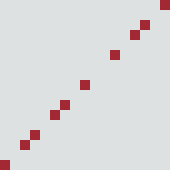
\includegraphics[width=37mm]{../../../output/profiling/emissive-gi/edge-current.png}\\[-1pt]
{\small 旧版 GPU 的 $17\times17$ 个交点}
\end{minipage}\hfill
\begin{minipage}[b]{.64\linewidth}\centering
\begin{tikzpicture}[x=1mm,y=1mm,every node/.style={font=\small,text=ink},>=Stealth]
\draw[rounded corners=2pt,draw=line] (0,0) rectangle (97,38);
\node[anchor=west,font=\small\bfseries,text=blue] at (3,34){从侧面看中心像素};
\fill[blue!8] (58,8) rectangle (79,25);
\draw[blue,thick] (58,8)--(58,25);
\draw[muted,thick] (79,8)--(79,25);
\draw[->,thick] (9,18)--(57.3,18);
\node[anchor=west] at (6,23){相机射线};
\draw[->,dashed,thick,red!55!black] (58,18)--(79,18);
\fill[blue] (58,18) circle[radius=1.1];
\fill[red!55!black] (79,18) circle[radius=1.1];
\node[font=\footnotesize,anchor=north] at (58,8){正面 $z=0$};
\node[font=\footnotesize,anchor=north] at (81,8){背面 $z=-0.1$};
\end{tikzpicture}\\[-1pt]
{\small 实线到达正面，虚线是旧版多走的一段}
\end{minipage}
\caption{左图按 Vulkan 读回的位置着色。灰格打到了正面，红格打到了背面；红色只标记错误。右图按项目墙面尺寸另绘，横向放大了厚度，箭头表示射线方向。}
\end{figure}

测试中墙宽和高都是 2.2。正交相机只看墙中央宽 0.5 的部分，向前发出 289 条平行射线。中心像素是第 8 列、第 8 行，从零开始计数。旧版在这里读到了 $z=-0.1$。其余九个错误像素也在同一条对角线上。旁边的像素读到约 $2.38\times10^{-7}$，这点误差远小于墙的厚度，可以确认打到的是正面。它也说明只看命中与否还不够：穿过去的射线同样命中了模型，只是表面错了。

旧代码先用射线和两个三角形分别计算重心坐标。把一个三角形的顶点记为 $A,B,C$，它内部的点可以写成 $(1-u-v)A+uB+vC$。三个权重都非负，点才在三角形内。刚好落在边上时，有一个权重应当等于零。

\loc{Redflag/src/Redflag/Renderer/GI/Shaders/Trace.glsl}
\begin{Code}
// 旧 trace：只要有一个权重小于零，这个三角形就不接受此次命中。
if (u < 0. || u > 1.) continue;
if (v < 0. || u + v > 1.) continue;
\end{Code}

对于接缝上的同一个点，两块三角形可能用不同顶点算出拼接边的位置。一边直接检查某个权重，另一边可能拿另外两个数相加，再同 1 比较。计算机能保存的小数位有限，两边各自舍入后，就可能同时把它排除。把相机水平移动 0.007 个场景单位，像素中心离开接缝，旧版的 289 条射线也能命中正面。先前的灯牌面积积分用过这个机位，本页专门把相机移回正中央。

普通编辑器用光栅化生成眼前的墙面。这里的射线检查用于从表面找反射光和遮挡物，测试专门读回这条路径的交点。用正交相机逐格发射，便于准确找到出错的那条边。\href{run:../profiling/emissive-gi/edge-current.csv}{旧版逐像素坐标}

\begin{figure}[H]\centering
\begin{tikzpicture}
\begin{axis}[width=.89\linewidth,height=27mm,scale only axis,
  xmin=-.7,xmax=16.7,xtick={0,4,8,12,16},xlabel={对角线上像素的列号},
  ymin=-.123,ymax=.035,ytick={-.1,0},yticklabels={$-0.1$,$0$},ylabel={$z$},
  axis lines=left,axis line style={draw=line},tick style={draw=muted},
  ymajorgrids=true,grid style={draw=line},tick label style={font=\footnotesize},
  label style={font=\footnotesize},legend style={at={(.98,.98)},anchor=north east,
    draw=none,fill=none,font=\footnotesize},legend columns=2]
\addplot[only marks,mark=o,mark size=2.7pt,blue,line width=.7pt]
  table[col sep=comma,x=x,y=new]{../../../output/profiling/emissive-gi/edge-diagonal.csv};
\addlegendentry{修正后}
\addplot[only marks,mark=x,mark size=2pt,red!60!black,line width=.7pt]
  table[col sep=comma,x=x,y=old]{../../../output/profiling/emissive-gi/edge-diagonal.csv};
\addlegendentry{修正前}
\end{axis}
\end{tikzpicture}
\caption{旧版和正式修正版本在相同镜头下逐像素读回的交点。十个红叉落在背面。修正后 17 个空心圆都在正面，整幅图的 289 条射线也全部通过。}
\end{figure}

\clearpage
\section{公共边的投影与交点}

可以让两块三角形用相同的算式检查同一条边。先把射线起点当作原点，再沿射线看过去。射线在眼前这张平面上变成一个点 $P$，两个三角形的公共边投影成线段 $AB$。我们只需检查 $P$ 在三条边的哪一侧。每个顶点都用同一条射线来投影，相邻三角形便可以直接使用相同的 $A$、$B$。

\begin{figure}[H]\centering
\begin{tikzpicture}[x=1mm,y=1mm,every node/.style={font=\small,text=ink},>=Stealth]
  \draw[rounded corners=2pt,draw=line] (0,0) rectangle (153,45);
  \draw[draw=blue,fill=blue!10] (10,7)--(50,7)--(50,37)--cycle;
  \draw[draw=blue,fill=warm] (10,7)--(50,37)--(10,37)--cycle;
  \draw[draw=ink,line width=.8pt] (10,7)--(50,37);
  \node[anchor=east] at (9,7){$A$};
  \node[anchor=west] at (51,37){$B$};
  \filldraw[draw=white,fill=red!55!black,line width=.6pt] (30,22) circle[radius=1.6];
  \node[above left,inner sep=2pt] at (30,22){$P$};
  \node[anchor=west,font=\small\bfseries,text=blue] at (60,34){从射线方向看，两块三角形共用 $AB$};
  \node[anchor=west] at (60,23){顺着 $A\rightarrow B$ 和 $B\rightarrow A$ 各检查一次。};
  \node[anchor=west] at (60,12){$P$ 在接缝上，与 $A,B$ 围出的面积均为 0。};
\end{tikzpicture}
\caption{沿射线方向投影的示意图，据 Woop 等人论文第 3 节的边测验绘制。暖色、蓝色各表示一个三角形。红点是射线投影到平面的位置。}
\end{figure}

投影后令 $P=(0,0)$。沿 $A\rightarrow B$ 检查得到 $E=A_x B_y-A_y B_x$，这是三点围成的有向面积的两倍。取 $A=(-1,-1),B=(1,1)$，算出 $E=-1-(-1)=0$。交换端点得到 $-E$。同样检查三条边，只要同时出现正数和负数，点就在三角形外；全为同一符号或有一项为零时，还要检查三角形是否有面积以及交点是否在射线规定的距离内。

\loc{Redflag/src/Redflag/Renderer/GI/Shaders/Trace.glsl}
\begin{Code}
// trace 中的 pa、pb、pc 是沿本条射线投影后的三个顶点。
vec3 areas = vec3(edgeArea(pb, pc), edgeArea(pc, pa), edgeArea(pa, pb));
if (any(lessThan(areas, vec3(0))) && any(greaterThan(areas, vec3(0)))) continue;
\end{Code}

传给 GPU 的 \code{GITriangle} 原来保存一个顶点 $A$ 和两条边向量 $B-A,\ C-A$。用它们还原 $B$ 时需要再做一次加法，其中一部分小数位可能在先前相减时已经丢失。现在把 $A,B,C$ 三个世界坐标直接保存下来，同一条边的端点就能用相同的数值参与两次判断。每个三角形仍占 64 字节。

计算有向面积时，着色器先分别保存两个乘积，再做减法。若两个乘积近得舍入成了同一个数，就用融合乘加（\code{fma}）分别取回它们舍掉的部分。这样一来，即使设备只用 32 位浮点数，也能分辨一部分原本会算成零的差值。论文还讨论了极端情况下使用双精度重新计算，本项目的适用范围由实测例子检验。

保留真实开口也很重要。把两片墙分开 0.002 个场景单位，正对缝隙的中心射线仍能穿过，左右相邻的射线都被墙挡住。再把一块挡板摆在白墙和点光源之间，白墙中央测到的线性红通道是 0。把挡板移到点光源后，或改成当前按透光处理的薄玻璃，那里都是 0.168192。这样能分别检查接缝、留给光线通过的空间和从墙到灯的遮挡范围。

在仓库根目录给 \path{tests/run_gi_benchmark.cmd} 传入 \code{--triangle-edge}。它还会把八片三角形拼成的墙转到三个坐标轴，从正面和背面各做两次检查，一次用正交相机，另一次用透视相机斜着看。这 12 个视角各测 289 条射线，3,468 个交点都落在预期面上。它们覆盖了这里列出的尺度和角度。\\
\href{run:../profiling/emissive-gi/edge-final.csv}{正式版本逐像素坐标}\quad
\href{run:../profiling/emissive-gi/edge-directions.csv}{各视角读数}\quad
\href{run:../../tests/TriangleIntersectionCheck.h}{真实缝隙与点光源测试}

\noindent\href{https://jcgt.org/published/0002/01/05/paper.pdf}{Woop、Benthin、Wald，JCGT 2013，第 3 节}\quad
\href{https://pbr-book.org/4ed/Shapes/Triangle_Meshes#TriangleIntersection}{PBRT 第四版 §6.5.3，射线与三角形求交}
